\documentclass[aspectratio=169]{beamer}
\usepackage{will_handley}
\usepackage{pythonhighlight}
\usepackage{tikz}
\usetikzlibrary[positioning]
\usetikzlibrary{calc}
\usetikzlibrary{fit}

\usepackage{listings}
 

% Commands
% --------
% - \arxiv{arxiv number}
% - \cols{width}{lh column}{rh column}
% -  \begin{fig(left|right)}[fractional width (e.g 0.6) ]{name of image}
%        content of other column
%    \end{fig(left|right)}

% Talk details
% ------------
\title{Next generation cosmological analysis with nested sampling}
\date{8\textsuperscript{th} September 2022}
\newcommand{\av}[2][]{\left\langle #2\right\rangle_{#1}}

\begin{document}

\begin{frame}
    \titlepage
\end{frame}

\begin{frame}
    \frametitle{Overview}
    \begin{columns}
        \column{0.5\textwidth}
        \begin{itemize}
            \item DiRAC 2020 RAC allocation of 30MCPUh
            \item Main goal: Planck Legacy Archive equivalent
                \vspace{-10pt}
                \begin{itemize}
                    \item Parameter estimation $\to$ Model comparison
                    \item MCMC $\to$ Nested sampling
                    \item Planck $\to$ $\{\text{Planck}, \text{DESY1}, \text{BAO}, \ldots \}$
                    \item Pairwise combinations
                \end{itemize}
            \item Suite of tools for processing these 
                \begin{itemize}
                    \item \texttt{unimpeded} $1.0$
                    \item \texttt{margarine} $1.0$
                    \item \texttt{anesthetic} $2.0$
                    \item \texttt{zenodo} archive
                \end{itemize}
            \item MCMC chains also available.
            \item Work in progress, but $\alpha$-testers requested (email \href{mailto:wh260@cam.ac.uk}{wh260@cam.ac.uk})
        \end{itemize}
        \column{0.5\textwidth}
        
\includegraphics[width=\textwidth]{logos/dirac}
        \includegraphics[width=0.5\textwidth,page=21]{figures/himmelblau}%
        \includegraphics[width=0.5\textwidth,page=15]{figures/himmelblau}
    \end{columns}
\end{frame}

\begin{frame}
    \frametitle{The three pillars of Bayesian inference}
    \begin{columns}[t]
        \column{0.33\textwidth}
        \begin{block}{Parameter estimation}
            What do the data tell us about the parameters of a model?

            \textit{e.g. the size or age of a $\Lambda$CDM universe}
            \[ \hspace{-10pt}\C[0]{P(\theta|D,M)} = \frac{\C[2]{P(D|\theta,M)} \C[1]{P(\theta|M)}}{\C[3]{P(D|M)}}, \] 
            \[ \C[0]{\mathcal{P}} = \frac{\C[2]{\mathcal{L}} \times\C[1]{\pi}}{\C[3]{\mathcal{Z}}}, \] 
            \[ \C[0]{\text{Posterior}} = \frac{\C[2]{\text{Likelihood}} \times\C[1]{\text{Prior}}}{\C[3]{\text{Evidence}}}. \]
        \end{block}
        \column{0.33\textwidth}
        \begin{block}{Model comparison}
            How much does the data support a particular model?

            \textit{e.g. $\Lambda$CDM vs a dynamic dark energy cosmology}
            \[ \C[4]{P(M|D)} = \frac{\C[3]{P(D|M)} \C[5]{P(M)}}{\C[7]{P(D)}}, \] \[ \frac{\C[3]{\mathcal{Z}_\mathcal{M}} \C[5]{\Pi_\mathcal{M}}}{\C[7]{\sum_m Z_m \Pi_m}}, \] \[ \C[4]{\text{Posterior}} = \frac{\C[3]{\text{Evidence}} \times\C[5]{\text{Prior}}}{\C[7]{\text{Normalisation}}}.\]
        \end{block}
        \column{0.33\textwidth}
        \begin{block}{Tension quantification}
            Do different datasets make consistent predictions from the same model? 

            \textit{e.g. CMB vs Type IA supernovae data}
            \[ \mathcal{R} = \frac{\C[3]{\mathcal{Z}}_{AB}}{\C[3]{\mathcal{Z}}_A\C[3]{\mathcal{Z}}_\mathcal{B}}, \] 
            \[
                \begin{aligned} \log\mathcal{S} = \av[{\C[0]{\mathcal{P}}_{AB}}]{\C[2]{\log\mathcal{L}}_{AB}}&\\
                    -\av[{\C[0]{\mathcal{P}}_{A}}]{\C[2]{\log\mathcal{L}}_{A}}&\\
                    -\av[{\C[0]{\mathcal{P}}_{B}}]{\C[2]{\log\mathcal{L}}_{B}}&
                \end{aligned}
            \]
        \end{block}
    \end{columns}
\end{frame}

\begin{frame}
    \frametitle{Occam's Razor~\arxiv{2102.11511}}
    \begin{itemize}
        \item Bayesian inference quantifies Occam's Razor:
            \begin{itemize}
                \item \textit{``Entities are not to be multiplied without necessity''} \hfill --- William of Occam
                \item \textit{``Everything should be kept as simple as possible, but not simpler''} \hfill --- ``Albert Einstein''
            \end{itemize}
        %\item Consider the Evidence $\C[3]{\mathcal{Z}\equiv P(D|M)}$: 
        %    \begin{description}[Parameter estimation]
        %        \item [Parameter estimation] normalisation constant
        %        \item [Model comparison] critical update factor for \C[5]{model prior} to \C[4]{model posterior}
        %    \end{description}
        \item Properties of the evidence: rearrange Bayes' theorem for parameter estimation
            \[\C[0]{\mathcal{P}(\theta)} = \frac{\C[2]{\mathcal{L}(\theta)} \C[1]{\pi(\theta)}}{\C[3]{\mathcal{Z}}} \qquad\Rightarrow\qquad \C[3]{\log \mathcal{Z}} = \C[2]{\log\mathcal{L}(\theta)} - \log \frac{\C[0]{\mathcal{P}(\theta)}}{\C[1]{\pi(\theta)}} \]  
        \item Evidence is composed of a ``goodness of fit'' term  and ``Occam Penalty''
    \end{itemize}
    \begin{columns}[t]
        \column{0.5\textwidth}
        \begin{itemize}
            \item RHS true for all $\theta$. Take max likelihood value $\theta_*$:
                \[
                    \C[3]{\log \mathcal{Z}} = -\chi_\mathrm{min}^2 - \text{Mackay penalty}
                \]
        \end{itemize}
        \column{0.5\textwidth}
        \begin{itemize}
            \item Be more Bayesian and take posterior average to get the ``Occam's razor equation''
                \[
                    \boxed{
                        \C[3]{\log \mathcal{Z}} = \av[{\C[0]{\mathcal{P}}}]{\C[2]{\log\mathcal{L}}} - \mathcal{D}_\mathrm{KL}
                    }
                \]
        \end{itemize}
    \end{columns}
    \vfill
    \begin{itemize}
        \item Natural regularisation which penalises models with too many parameters.
    \end{itemize}
\end{frame}

\begin{frame}
    \frametitle{Kullback Liebler divergence}
    \begin{columns}
        \column{0.5\textwidth}
        \begin{itemize}
            \item The KL divergence between \C[1]{prior $\pi$} and \C[0]{posterior $\mathcal{P}$} is defined as:
                \[\mathcal{D}_\mathrm{KL} = \av[{\C[0]{\mathcal{P}}}]{\log\frac{\C[0]{\mathcal{P}}}{\C[1]{\pi}}} = \int \C[0]{\mathcal{P}(\theta)} \log \frac{\C[0]{\mathcal{P}(\theta)}}{\C[1]{\pi(\theta)}}d\theta.\]
            \item Whilst not a distance, $\mathcal{D}=0$ when $\C[0]{\mathcal{P}}=\C[1]{\pi}$.
            \item Occurs in the context of machine learning as an objective function for training functions.
            \item In Bayesian inference it can be understood as a log-ratio of ``volumes'':
                \[ \mathcal{D}_\mathrm{KL} \approx \log \frac{\C[1]{V_\pi}}{\C[0]{V_\mathcal{P}}}.\]
                (this is exact for top-hat distributions).
        \end{itemize}
        \column{0.5\textwidth}
        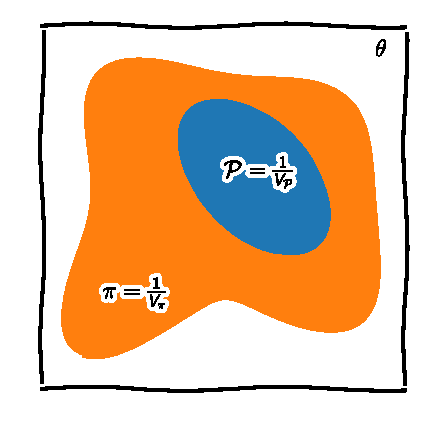
\includegraphics{figures/volumes.pdf}
    \end{columns}
\end{frame}

\begin{frame}
    \frametitle{Why do sampling?}
    \begin{columns}
        \column{0.5\textwidth}
        \begin{itemize}
            \item The cornerstone of numerical Bayesian inference is working with \textbf{samples}.
            \item Generate a set of representative parameters drawn in proportion to the posterior $\theta\sim\C[0]{\mathcal{P}}$.
            \item The magic of marginalisation $\Rightarrow$ perform usual analysis on each sample in turn.
            \item The golden rule is \C[3]{stay in samples} until the last moment before computing summary statistics/triangle plots because \[\boxed{f(\:\av{X}\:)\ne \av{\:f(X)\:}}\]
            \item Generally need $\sim\mathcal{O}(12)$ independent samples to compute a value and error bar.
        \end{itemize}
        \column{0.5\textwidth}
        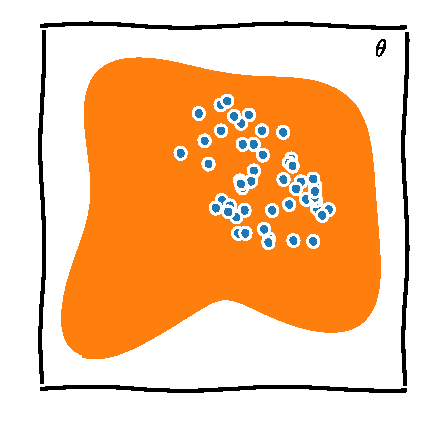
\includegraphics{figures/samples.pdf}
    \end{columns}
\end{frame}

\begin{frame}
    \frametitle{The Planck legacy archive}
    \begin{columns}
        \column{0.5\textwidth}
        \begin{itemize}
            \item \textit{Planck} collaboration science products
            \item Distributed cosmology inference results as MCMC chains
            \item Across a grid of:
                \begin{itemize}
                    \item subsets/combinations of \textit{Planck} data
                        \begin{itemize}
                            \item TT, lowl, lowE, lensing
                        \end{itemize}
                    \item $\Lambda$CDM extensions 
                        \begin{itemize}
                            \item base, mnu, nrun, omegak, r
                        \end{itemize}
                \end{itemize}
            \item importance sampling across some other likelihoods (BAO, JLA,\ldots)
            \item Cannot compute evidences in high dimensions from MCMC chains
                \begin{itemize}
                    \item Only parameter estimation
                    \item no model comparison
                \end{itemize}
        \end{itemize}
        \column{0.5\textwidth}
        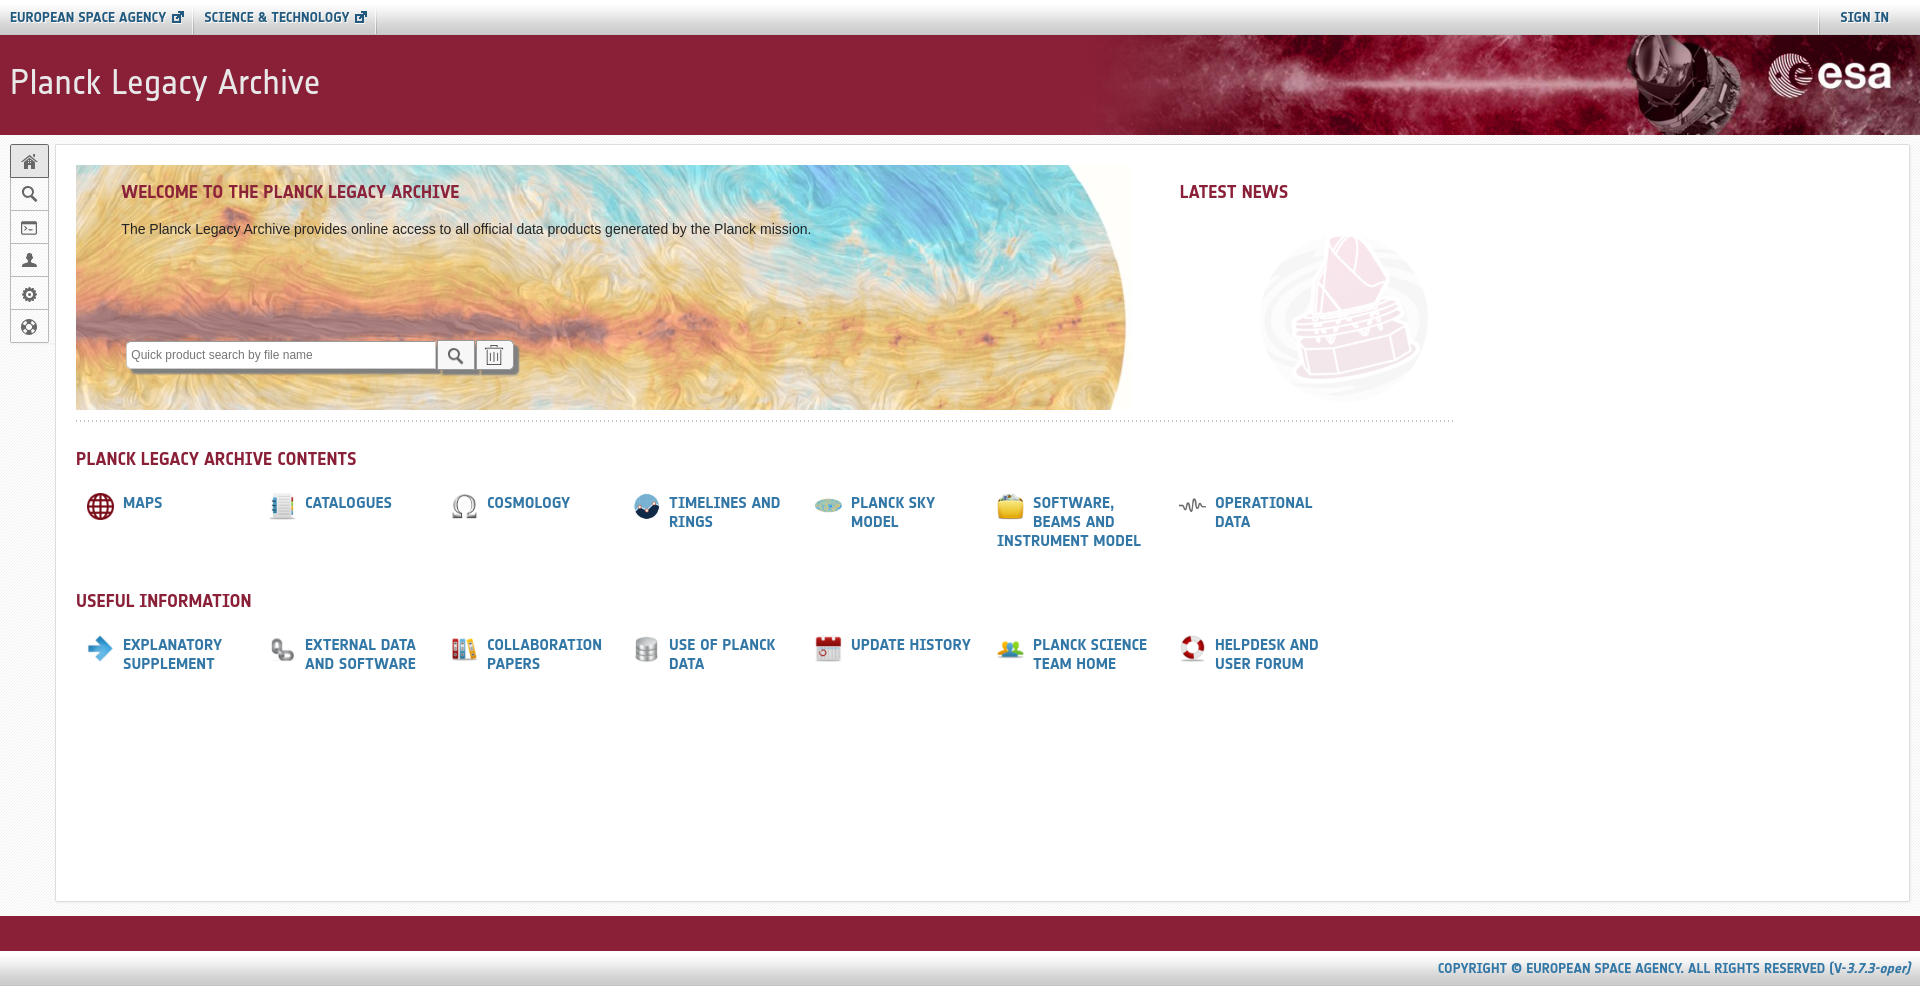
\includegraphics[width=\textwidth]{figures/pla}
        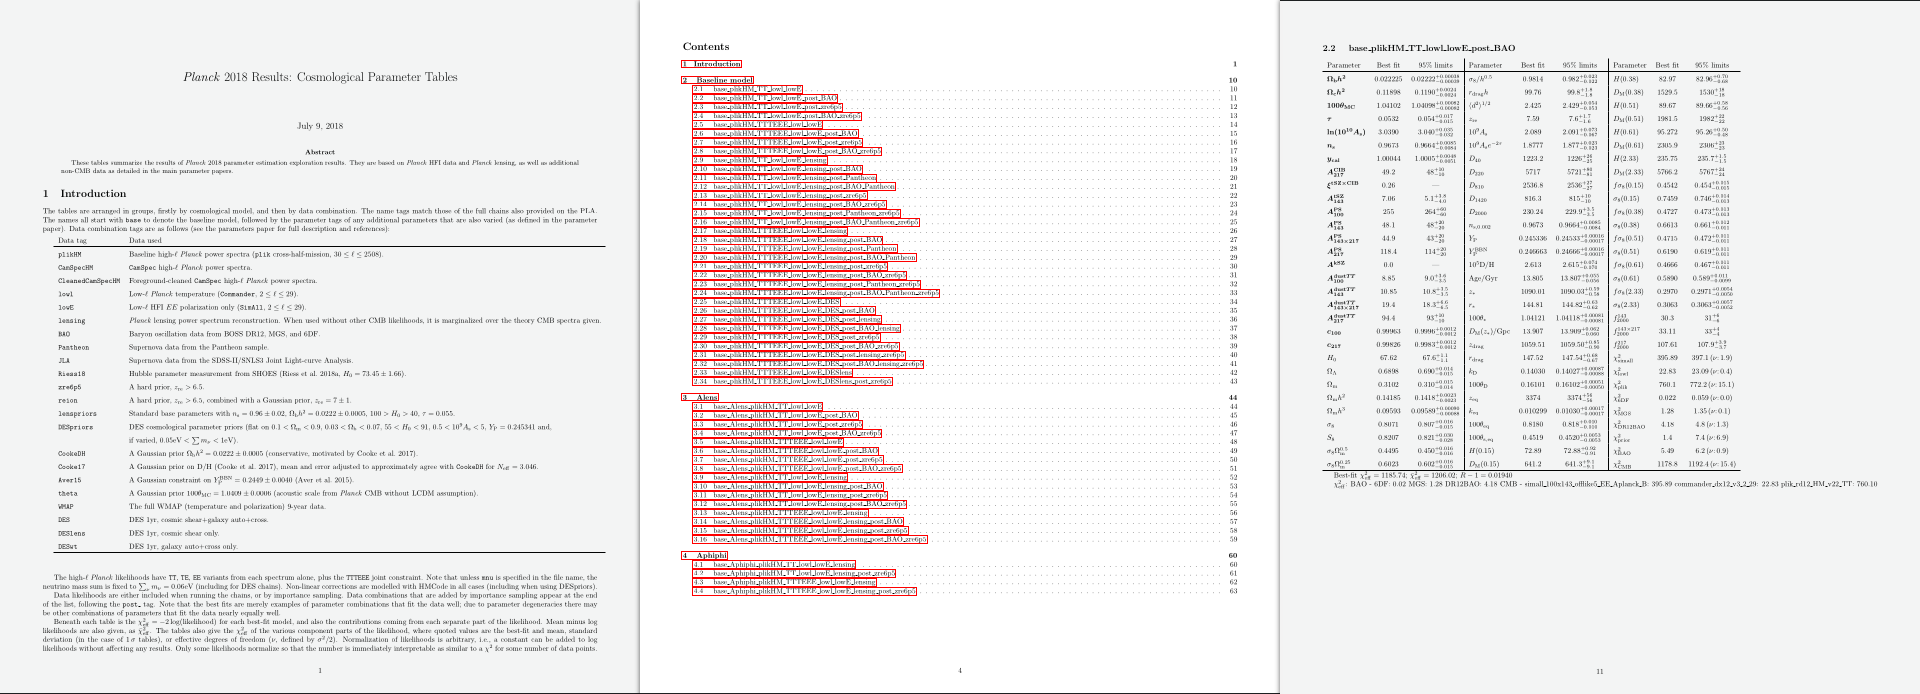
\includegraphics[width=\textwidth]{figures/pla1}
    \end{columns}
\end{frame}

\begin{frame}
    \begin{columns}
        \column{0.5\textwidth}
        \begin{block}{\textbf{MCMC}}
            \includegraphics<1>[width=\textwidth,page=16]{figures/himmelblau}%
            \includegraphics<2>[width=\textwidth,page=17]{figures/himmelblau}%
            \includegraphics<3>[width=\textwidth,page=18]{figures/himmelblau}%
            \includegraphics<4>[width=\textwidth,page=19]{figures/himmelblau}%
            \includegraphics<5>[width=\textwidth,page=20]{figures/himmelblau}%
            \includegraphics<6-15>[width=\textwidth,page=21]{figures/himmelblau}%
            \begin{itemize}
                \item<16> Single ``walker''
                \item<16> Explores posterior
                \item<16> Fast, if proposal matrix is tuned
                \item<16> Parameter estimation, suspiciousness calculation
                \item<16> Channel capacity optimised for generating posterior samples
            \end{itemize}
        \end{block}
        \centerline{\includegraphics<16>[width=0.5\textwidth,page=19]{figures/himmelblau}}
        \column{0.5\textwidth}
        \begin{block}<7->{\textbf{Nested sampling}}
            \includegraphics<7|handout:0>[width=\textwidth,page=1]{figures/himmelblau}%
            \includegraphics<8|handout:0>[width=\textwidth,page=2]{figures/himmelblau}%
            \includegraphics<9|handout:0>[width=\textwidth,page=3]{figures/himmelblau}%
            \includegraphics<10          >[width=\textwidth,page=4]{figures/himmelblau}%
            \includegraphics<11|handout:0>[width=\textwidth,page=5]{figures/himmelblau}%
            \includegraphics<12|handout:0>[width=\textwidth,page=6]{figures/himmelblau}%
            \includegraphics<13|handout:0>[width=\textwidth,page=7]{figures/himmelblau}%
            \includegraphics<14|handout:0>[width=\textwidth,page=8]{figures/himmelblau}%
            \includegraphics<15|handout:0>[width=\textwidth,page=15]{figures/himmelblau}%
            \begin{itemize}
                \item<16> Ensemble of ``live points''
                \item<16> Scans from prior to peak of likelihood
                \item<16> Slower, no tuning required
                \item<16> Parameter estimation, model comparison, tension quantification
                \item<16> Channel capacity optimised for computing partition function
            \end{itemize}
        \centerline{\includegraphics<16>[width=0.5\textwidth,page=4]{figures/himmelblau}} \end{block}
    \end{columns}
\end{frame}

\begin{frame}
    \frametitle{The grid (so far)}
        \begin{itemize}
            \item Models: $[\Lambda\text{CDM}, \Omega_K, \nu, r, w, w(a)]$
            \item Data: [\texttt{plik}, \texttt{camspec}, \texttt{DESY1}, \texttt{bicep+keck}, \texttt{BAO(DR16)}, \texttt{pantheon} ]
            \item Pairwise combinations of datasets
            \item Breakdown of Planck \& BAO data
            \item Samplers: [Metropolis Hastings MCMC, Nested Sampling]
            \item These exhaust what is currently available by default in $\texttt{cobaya}$
            \item Wide priors to allow for importance readjustment as desired
            \item roughly halfway through computational allocation. 
            \item Feedback desirable as to what extensions to the grid would be of community interest (email \href{mailto:wh260@cam.ac.uk}{wh260@cam.ac.uk}) (\texttt{Pantheon+}, S$H_0$ES, \texttt{NPIPE}, \texttt{DESY3},\ldots).
            \item Further checking needed before first release by end of this year.
        \end{itemize}
\end{frame}

\begin{frame}[fragile]
    \frametitle{\texttt{unimpeded}}
    \framesubtitle{Universal Model comparison and Parameter Estimation Distributed over Every Dataset}
    \begin{columns}
        \column{0.5\textwidth}
    \begin{itemize}
        \item Python tool for seamlessly downloading, uploading and cacheing of chains
        \item Data stored on \texttt{zenodo} 
        \item hdf5 storage for fast \& reliable storage
        \item \texttt{anesthetic} compatible for processing of chains~\arxiv{1905.04768}
        \item $\alpha$-testers wanted! (email \href{mailto:wh260@cam.ac.uk}{wh260@cam.ac.uk}) 
        \item End goal -- community library which everyone contributes to so expensive inference products are reusable and reused.
    \end{itemize}
        \column{0.5\textwidth}


\lstset{language=Python}
\lstset{frame=lines}
\lstset{basicstyle=\footnotesize}
\begin{lstlisting}
from unimpeded import Unimpeded
store = Unimpeded(cache='data.hdf5')
samps = store('planck')
samps.H0.plot.kde_1d()
samps = store('planck', model='klcdm')
samps.H0.plot.kde_1d()
\end{lstlisting}
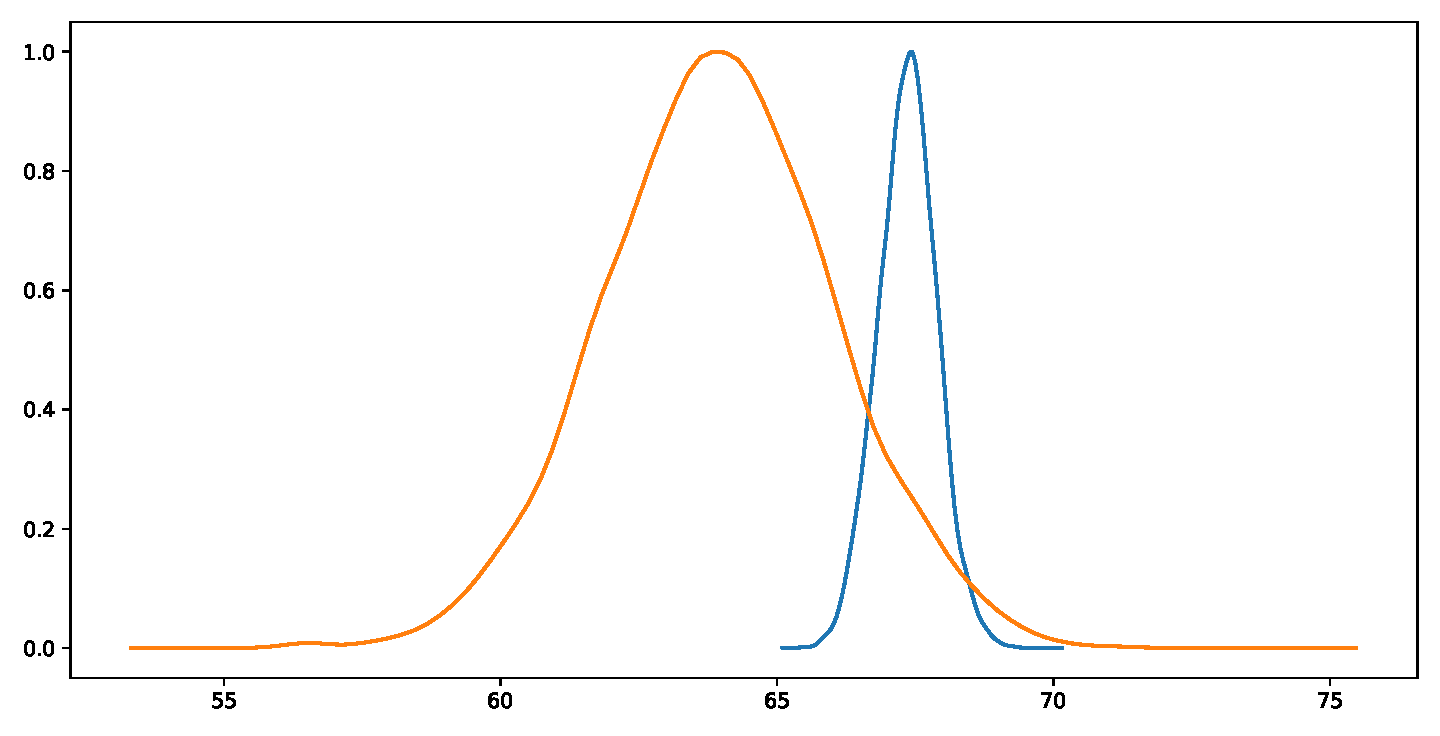
\includegraphics[width=\textwidth]{figures/unimpeded.pdf}

        
    \end{columns}
\end{frame}

%\begin{frame}
%\begin{tikzpicture}[rednode/.style={rectangle, draw=red!60, fill=red!5, very thick, minimum size=5mm},
%bluenode/.style={rectangle, draw=blue!60, fill=blue!5, very thick, minimum size=5mm},
%remember picture, overlay]
%
%\node<1->[bluenode](likelihoodA) at (1,2) {$ \mathcal{L}_A(\theta,\alpha_A)$};
%\node<1->[bluenode, right = 0 of likelihoodA.east](likelihoodB) {$ \mathcal{L}_B(\theta,\alpha_B)$};
%\node<2->[bluenode, below = of likelihoodB.west](likelihoodAB) {$ \mathcal{L}_A(\theta,\alpha_A) \mathcal{L}_B(\theta,\alpha_B)$};
%
%
%\draw<2->[->] (likelihoodA.south) -- (likelihoodA.south |- likelihoodAB.north);
%\draw<2->[->] (likelihoodB.south) -- (likelihoodB.south |- likelihoodAB.north);
%
%\node<3->[bluenode, right = 0 of likelihoodAB.east](prior) {$ \pi_{AB}(\theta,\alpha_A, \alpha_B)$};
%
%\node<4->[rednode, align=center, below = of likelihoodAB.east](nestedsampling)  {Nested Sampling with $\theta$, $\alpha_A$ and $\alpha_B$};
%
%\draw<4->[->] (likelihoodAB.south) -- (likelihoodAB.south |- nestedsampling.north);
%\draw<4->[->] (prior.south) -- (prior.south |- nestedsampling.north);
%
%
%\node<5->[bluenode, below = of nestedsampling.south](jointPosterior2) {$ \{\theta,\alpha_A,\alpha_B\}_{\mathcal{P}_{AB}}$};
%\draw<5->[->] (nestedsampling.south) -- (jointPosterior2.north);
%
%\node<6->[bluenode, below = of jointPosterior2.south](jointPosterior1) {$ \{\theta\}_{\mathcal{P}_{AB}}$};
%
%\draw<6->[->] (jointPosterior2.south) -- (jointPosterior1.north);
%
%\node<7->[bluenode,  right = of jointPosterior1.east](jointEvidence2) {$ \mathcal{Z}_{AB}$};
%\draw<7->[->] (nestedsampling.south-|jointEvidence2.north) -- (jointEvidence2.north);
%
%
%
%\end{tikzpicture}
%\end{frame}

%\begin{frame}
%\begin{tikzpicture}[squarednodeA/.style={rectangle, draw=red!60, fill=red!5, very thick, minimum size=5mm},
%squarednodeB/.style={rectangle, draw=blue!60, fill=blue!5, very thick, minimum size=5mm},
%squarednodeC/.style={rectangle, draw=green!60, fill=green!5, very thick, minimum size=5mm}]
%
%\node[squarednodeB](likelihood1) at (6, 1.5){$ \mathcal{L}_A(\theta,\alpha_A)$};
%\node[squarednodeB](prior1) at (8, 1.5){$ \pi_A(\theta,\alpha_A)$};
%
%\node[squarednodeC, text width=3cm, align=center](NestedMarg1) at (7, 0){Nested Sampling + \texttt{margarine}};
%
%\draw[->](likelihood1.south) -- (6, 0.5);
%\draw[->](prior1.south) -- (8, 0.5);
%
%\node[squarednodeB](marglike1) at (6, -1.5){$ \mathcal{L}_A(\theta)$};
%\node[squarednodeB](margprior1) at (9, -1.5){$ \pi(\theta)$};
%
%\draw[->](6, -0.5) -- (6, -1.2);
%\draw[->](8, -0.5) -- (9, -1.2);
%
%\node[squarednodeB](likelihood2) at (10, 1.5){$ \mathcal{L}_B(\theta,\alpha_B)$};
%\node[squarednodeB](prior2) at (12, 1.5){$ \pi_B(\theta,\alpha_B)$};
%
%\draw[->](likelihood2.south) -- (10, 0.5);
%\draw[->](prior2.south) -- (12, 0.5);
%
%\node[squarednodeC, text width=3cm, align=center](NestedMarg1) at (11, 0){Nested Sampling + \texttt{margarine}};
%
%\node[squarednodeB](marglike2) at (12, -1.5){$ \mathcal{L}_B(\theta)$};
%\draw[->](12, -0.5) -- (12, -1.2);
%\draw[->](10, -0.5) -- (9, -1.2);
%
%\node[squarednodeB](combinedlike) at (7, -3){$ \mathcal{L}_A(\theta) \mathcal{L}_B(\theta)$};
%
%\draw[->](marglike1.south) -- (combinedlike.north);
%\draw[->](marglike2.south) -- (combinedlike.north);
%
%\node[squarednodeA, text width=3cm, align=center](inference2) at (9, -4.5) {Nested Sampling with $\theta$};
%
%\draw[->](combinedlike.south) -- (8, -4);
%\draw[->](margprior1.south) -- (10, -4);
%
%\node[squarednodeB](jointEvidence) at (8, -6){$ \mathcal{Z}_{AB}$};
%\node[squarednodeB](jointPosterior) at (10, -6){$ \{\theta\}_{\mathcal{P}_{AB}}$};
%
%\draw[->](8, -5) -- (jointEvidence.north);
%\draw[->](10, -5) -- (jointPosterior.north);
%\end{tikzpicture}
%\end{frame}

\begin{frame}
    \frametitle{\texttt{margarine}: machine learning-enhanced Bayesian inference}
    %\begin{tikzpicture}[remember picture,overlay]
    %    \node (student) [xshift=-0.11\textwidth,yshift=-0.18\textwidth] at (current page.north east) {
\includegraphics[width=0.2\textwidth]{figures/harry_bevins.jpg}};
    %    \node[below=0 of student.south,align=center]{Harry Bevins\\\arxiv{2207.11457}};
    %\end{tikzpicture}

    \begin{columns}
        \column{0.6\textwidth}
        \begin{columns}
            \column{0.3\textwidth}
            
\includegraphics[width=\textwidth]{figures/harry_bevins.jpg}
            Harry Bevins \\ \arxiv{2205.12841} \\ \arxiv{2207.11457}
            \column{0.7\textwidth}
            \begin{itemize}
                \item Can use machine learning + grid to dramatically speed up inference
                \item Emulate the marginal posterior and prior with  masked autoregressive flows (\texttt{margarine})
                \item Use nested sampling evidences to compute nuisance marginalised likelihood $\mathcal{L}(\theta) = \mathcal{P}(\theta) \mathcal{Z}/\pi(\theta)$
            \end{itemize}
        \end{columns}
        \vspace{5pt}

        \begin{itemize}
            \item Library of pre-trained bijectors to be used as priors/emulators/nuisance marginalised likelihoods
            \item e.g. easy to apply a \textit{Planck}/DES/HERA/JWST prior or likelihood to your existing MCMC chains without needing to install the whole cosmology machinery.
        \end{itemize}

        \column{0.4\textwidth}
        \begin{tikzpicture}[
                rednode/.style={rectangle, draw=red!60, fill=red!5, very thick, minimum size=5mm},
                bluenode/.style={rectangle, draw=blue!60, fill=blue!5, very thick, minimum size=5mm},
                greennode/.style={rectangle, draw=green!60, very thick, minimum size=5mm},
                node distance=0.5cm,
                remember picture, overlay
            ]
            \node<2->[bluenode, xshift=0.5\textwidth, yshift=-0.25\textwidth](likelihood) at (current page.north)  {$ \mathcal{L}(\theta,\alpha)$};
            \node<3->[bluenode, right = of likelihood.east](prior) {$ \pi(\theta,\alpha)$};

            \coordinate<3-> (likelihoodprior) at ($(likelihood.south)!0.5!(prior.south)$);

            \node<4->[rednode, below = of likelihoodprior](nestedsampling) {Nested Sampling};
            \draw<4->[->](likelihood.south) -- (likelihood|-nestedsampling.north);
            \draw<4->[->](prior.south) -- (prior|-nestedsampling.north);

            \node<5->[bluenode, below = of nestedsampling](posterior) {$ \{\theta,\alpha\}_\mathcal{P}$};
            \draw<5->[->](nestedsampling.south-|posterior) -- (posterior.north);
            \node<6->[bluenode, left = of posterior.west](evidence) {$ \mathcal{Z}$};
            \draw<6->[->](nestedsampling.south-|likelihood) -- (evidence.north);
            \node<7->[bluenode, right = of posterior.east](priorSamples) {$ \{\theta,\alpha\}_\pi$};
            \draw<7->[->](nestedsampling.south-|prior) -- (priorSamples.north);

            \coordinate<7-> (posteriorprior) at ($(posterior.south)!0.5!(priorSamples.south)$);

            \node<8->[rednode, below = of posteriorprior](margarine)  {\texttt{margarine}};

            \draw<8->[->](posterior.south) -- (margarine.north-|posterior.east);
            \draw<8->[->](priorSamples.south) -- (margarine.north-|priorSamples.west);

            \node<9->[bluenode, below = of posterior|-margarine.south](marginalPosterior) {$ \mathcal{P}_\text{emu}(\theta)$};


            \draw<9->[->](margarine.south-|marginalPosterior.east) -- (marginalPosterior.north);


            \node<10->[bluenode, below = of marginalPosterior.south-|margarine.south-|priorSamples](marginalPrior) {$ \pi_\text{emu}(\theta)$};
            \draw<10->[->](margarine.south-|priorSamples.west) -- (marginalPrior.north);


            \node<11->[bluenode, below = of marginalPosterior](marginalLikelihood) {$ \mathcal{L}_\text{emu}(\theta)$};


            \draw<11->[->](evidence.south) -- (marginalLikelihood.west);
            \draw<11->[->](marginalPosterior.south) -- (marginalLikelihood.north);
            \draw<11->[->](marginalPrior.west) -- (marginalLikelihood.east);

            \node<12->[greennode,behind path,fit=(nestedsampling) (marginalPosterior) (priorSamples) (evidence),] {};

        \end{tikzpicture}
    \end{columns}
\end{frame}


\begin{frame}
    \frametitle{Conclusions}
    \begin{itemize}
        \item DiRAC RAC allocation for building a legacy grid of
            \begin{itemize}
                \item MCMC \& Nested sampling chains
                \item gridded over (pairwise) up-to-date datasets
                \item gridded over extensions to $\Lambda$CDM
                \item Bijectors \& emulators for fast re-use
                \item Importance sampling toolkit via \texttt{anesthetic} for (re)processing
                \item Long-term goal: community repository of chains to share model comparison compute resource
            \end{itemize}
        \item Looking for:
            \begin{itemize}
                \item $\alpha$-testers for \texttt{unimpeded}
                \item Suggestions for more datasets (and their incorporation into \texttt{cobaya})
            \end{itemize}
    \end{itemize}
\end{frame}

\end{document}
